\textbf{مورد استفاده:}
دریافت هزینه انجام پروژه
\\
\textbf{شرح مختصر :UC}
در این قسمت فریلنسر هزینه پروژه را دریافت می‌کند.
\\
\textbf{پيش شرط:}
ورود به مدیریت مالی در داشبورد فریلنسر.
\\
\textbf{سناريو اصلی:}
\begin{enumerate}
\item
شروع
\item
فریلنسر دکمه دریافت هزینه پروژه را انتخاب می‌کند و پروژه  انجام شده را در سایت بارگذاری می‌کند.
\item
کارفرما پروژه را تست/رویت و نظر خود را با دکمه ثبت نظر ثبت می‌کند.
\item
پس از تایید/لغو طرفین، پول بلوکه شده آزاد و به حساب فریلنسر/کارفرما واریز می‌شود.
\item
پروژه خاتمه یافتنه و در بانک اطلاعات ثبت می‌شود.
\item
پایان
\end{enumerate}

\noindent
\textbf{پس شرط:}
ندارد.
\\
\textbf{سناريوهای فرعی:}
\\
\textbf{سناريو فرعی 1:}
اصلاحات پروژه
\\
\textbf{شرح مختصر :UC}
این سناریو در مرحله 3 سناریو اصلی کارفرما بخش‌های نیاز به اصلاح را به فریلنسر اعلام می‌کند.
\begin{enumerate}
\item
شروع
\item
اصلاحات مورد نظر کارفرما طبق جهارچوب و قوانین سایت به فریلنسر جهت اعمال اعلام می‌شود.
\item
از مرحله 3 سناریو اصلی ادامه پیدا می‌کند.
\item
پایان
\end{enumerate}

\noindent
\textbf{سناريو فرعی 2:}
شکایت
\\
\textbf{شرح مختصر :UC}
این سناریو در مرحله ۴ سناریو اصلی در صورت شکایت طرفین اجرا می‌شود.
\begin{enumerate}
\item
شروع
\item
یکی از طرفین دکمه ثبت شکایت را انتخاب می‌کند و توضیحات شکایت خود را ثبت می‌کند.
\item
کارشناسان سایت به پروژه ورود کرده و نظر خود را در رابطه با آن اعلام می‌کنند.
\item
پس از لغو/تایید پروژه، از مرحله ۴ سناریو اصلی ادامه پیدا می‌کند.
\item
پایان
\end{enumerate}

\noindent
\textbf{پس شرط:}
ندارد.



\begin{figure}[H]
	\includegraphics[width=.7\textwidth]{Diagram/2.Activity/فریلنسر/مدیریت-مالی-دریافت.png}
	\centering
	\caption{دیاگرام فعالیت دریافت وجه}
	\label{fig:a:دریافت-وجه}
\end{figure}
\begin{figure}[H]
	\includegraphics[width=.7\textwidth]{Diagram/3.StateMachine/فریلنسر/مدیریت-مالی-دریافت.png}
	\centering
	\caption{دیاگرام حالت ماشین دریافت وجه}
	\label{fig:sm:دریافت-وجه}
\end{figure}
\begin{figure}[H]
	\includegraphics[width=1\textwidth]{Diagram/4.Collaboration/1.Sequence/فریلنسر/مدیریت-مالی-دریافت.png}
	\caption{دیاگرام توالی دریافت وجه}
	\centering
	\label{fig:s:دریافت-وجه}
\end{figure}
\begin{figure}[H]
	\includegraphics[width=1\textwidth]{Diagram/4.Collaboration/2.Communication/فریلنسر/مدیریت-مالی-دریافت.png}
	\centering
	\caption{دیاگرام همکار دریافت وجه}
	\label{fig:c:دریافت-وجه}
\end{figure}
